\documentclass[12pt,]{article}
\usepackage{lineno}
\usepackage[left=1in,top=1in,right=1in,bottom=1in]{geometry}
\newcommand*{\authorfont}{\fontfamily{phv}\selectfont}
\usepackage[]{mathpazo}

\usepackage[normalem]{ulem}
\useunder{\uline}{\ul}{}


  \usepackage[T1]{fontenc}
  \usepackage[utf8]{inputenc}



\usepackage{abstract}
\renewcommand{\abstractname}{}    % clear the title
\renewcommand{\absnamepos}{empty} % originally center

\renewenvironment{abstract}
 {{%
    \setlength{\leftmargin}{0mm}
    \setlength{\rightmargin}{\leftmargin}%
  }%
  \relax}
 {\endlist}

\makeatletter
\def\@maketitle{%
  \newpage
%  \null
%  \vskip 2em%
%  \begin{center}%
  \let \footnote \thanks
    {\fontsize{18}{20}\selectfont\raggedright  \setlength{\parindent}{0pt} \@title \par}%
}
%\fi
\makeatother




\setcounter{secnumdepth}{0}


\usepackage{graphicx,grffile}
\makeatletter
\def\maxwidth{\ifdim\Gin@nat@width>\linewidth\linewidth\else\Gin@nat@width\fi}
\def\maxheight{\ifdim\Gin@nat@height>\textheight\textheight\else\Gin@nat@height\fi}
\makeatother
% Scale images if necessary, so that they will not overflow the page
% margins by default, and it is still possible to overwrite the defaults
% using explicit options in \includegraphics[width, height, ...]{}
\setkeys{Gin}{width=\maxwidth,height=\maxheight,keepaspectratio}

\title{Temperature-dependent competition in container breeding mosquito species  }



\author{\Large Michelle V. Evans\vspace{0.05in} \newline\normalsize\emph{Odum School of Ecology, University of Georgia}  }


\date{}

\usepackage{titlesec}

\titleformat*{\section}{\normalsize\bfseries}
\titleformat*{\subsection}{\normalsize\itshape}
\titleformat*{\subsubsection}{\normalsize\itshape}
\titleformat*{\paragraph}{\normalsize\itshape}
\titleformat*{\subparagraph}{\normalsize\itshape}


\usepackage{natbib}
\bibliographystyle{ecolLet}
\usepackage[strings]{underscore} % protect underscores in most circumstances



\newtheorem{hypothesis}{Hypothesis}
\usepackage{setspace}

\makeatletter
\@ifpackageloaded{hyperref}{}{%
\ifxetex
  \PassOptionsToPackage{hyphens}{url}\usepackage[setpagesize=false, % page size defined by xetex
              unicode=false, % unicode breaks when used with xetex
              xetex]{hyperref}
\else
  \PassOptionsToPackage{hyphens}{url}\usepackage[unicode=true]{hyperref}
\fi
}

\@ifpackageloaded{color}{
    \PassOptionsToPackage{usenames,dvipsnames}{color}
}{%
    \usepackage[usenames,dvipsnames]{color}
}
\makeatother
\hypersetup{breaklinks=true,
            bookmarks=true,
            pdfauthor={Michelle V. Evans (Odum School of Ecology, University of Georgia)},
             pdfkeywords = {competition, mosquitoes, abiotic-biotic interactions, Ae. aegypti, An.
stephenshi},
            pdftitle={Temperature-dependent competition in container breeding mosquito species},
            colorlinks=true,
            citecolor=blue,
            urlcolor=blue,
            linkcolor=magenta,
            pdfborder={0 0 0}}
\urlstyle{same}  % don't use monospace font for urls

% set default figure placement to htbp
\makeatletter
\def\fps@figure{htbp}
\makeatother



% add tightlist ----------
\providecommand{\tightlist}{%
\setlength{\itemsep}{0pt}\setlength{\parskip}{0pt}}

\begin{document}

% \pagenumbering{arabic}% resets `page` counter to 1
%
% \maketitle

{% \usefont{T1}{pnc}{m}{n}
\setlength{\parindent}{0pt}
\thispagestyle{plain}
{\fontsize{18}{20}\selectfont\raggedright
\maketitle  % title \par

}

{
   \vskip 13.5pt\relax \normalsize\fontsize{11}{12}
\textbf{\authorfont Michelle V. Evans} \hskip 15pt \emph{\small Odum School of Ecology, University of Georgia}

}

}








\begin{abstract}

    \hbox{\vrule height .2pt width 39.14pc}

    \vskip 8.5pt % \small

\noindent Mosquito-borne disease has been increasing in recent decades, prompting
a proliferation of predictiong models of disease risk. Given the strong
relationship between many mosquito life-history traits and temperature,
the majority of these models predict mosquito dynamics as a function of
temperature, an abiotic factor, on the assumption that it is relatively
more important than biotic factors, such as species competition.
However, many mosquito species, particularly container-breeders, share
habitats at high densities, and is unknown what effect both intra and
interspecific compeittion may have on population growth rates. Here, we
explore the interactive effects of interspecific competition,
intraspecific competition, and temperature on the population growth of
two co-habiting mosquito species, \emph{Aedes aegypti} and
\emph{Anopheles stephensi}, using a laboratory model system to
parameterize demographic life history traits and calculate population
growth rates. We find that both species' population growth rates are a
function of both abiotic and biotic factors, but that an interaction
between the two is rare. Given their importance, future models of
mosquito dynamics should include both biotic and abiotic variables.


\vskip 8.5pt \noindent \emph{Keywords}: competition, mosquitoes, abiotic-biotic interactions, Ae. aegypti, An. stephensi \par

    \hbox{\vrule height .2pt width 39.14pc}



\end{abstract}


\vskip 6.5pt

\newpage

\noindent \doublespacing \linenumbers \section{Introduction}\label{introduction}

The frequency of infectious disease emergence has been increasing since
the mid-20th century. Incidence of vector borne diseases, specifically,
have increased over 25\% over the past decade \citep{jones2008}, with
notable recent outbreaks such as Zika and chikungunya in the Americas.
One driver of this increase is land-use change, such as agricultural
intensification and urbanization \citep{gottdenker2014, jones2013}.
Urbanization can cause increases in vector-borne disease through changes
to mosquito habitat and environmental conditions. For container breeding
species such as \emph{Aedes aegypti}, the primary vector of dengue and
yellow fever, urbanization increases the amount of habitat available for
breeding \citep{zahouli2017, li2014}. Further, urbanization can alter
the microclimate of the environment through the urban heat island
effect, leader to warmer temperatures in urban areas\citep{peng2012}.

Mosquitoes, being small ectotherms, are extremely susceptible to changes
in temperature, which can significantly impact on life history traits
relevant to demography and disease transmission
\citep{murdock2017, paaijmans2009}. The majority of past work has
focused on the abiotic effects of urbanization, ignoring changes to
biotic factors such as community composition and larval densities.
Mosquito population growth is density dependent in the larval stage
\citep{juliano1998, reiskind2009a}, and can be mediated by environmental
factors such as temperature \citep{costanzo2005, lounibos2002a} ,
leading to a potential interaction between abiotic and biotic factors,
defined as context-dependent competition.

Many primary vectors of arboviruses are container breeding species,
which often cohabit in containers with other mosquito species, leading
to strong control via density-dependence and interspecific competition
\citep{juliano2010}. For example, the invasion of the Southeastern
United States by \emph{Ae. albopictus} has lead to habitat partitioning
with \emph{Ae. aeygypti}, due to \emph{Ae. albopictus}'s competitive
dominance at low resource levels \citep{fader2016}. In this case, the
vectors share many pathogens, and the dominance of an area by one
species is not likely to introduce novel arboviruses to the population.
However, in some systems, cohabiting vectors may transmit different
pathogens, and competitive outcomes can have significant impacts on
disease transmission. In urban India, for example, \emph{Anopheles
stephensi}, the primary vector of urban malaria, is often found
cohabiting with \emph{Ae. aegypti}, the primary vector of dengue
\citep{thomas2016}. Both diseases have strong seasonal trends, due to
seasonality in temperature and rainfall \citep{santos-vega2016a}. This
seasonality of disease may be further mediated by competition between
the vectors of the diseases, however, the outcome of competition between
\emph{An. stephensi} and \emph{Ae. aeygypti}, and the extent to which it
is seasonally dependent is unknown.

Here, we explore the interactive effects of interspecific competition,
intraspecific competition, and temperature on the population growth of
two co-habiting mosquito species, \emph{Aedes aegypti} and
\emph{Anopheles stephensi}, using a laboratory model system to
parameterize demographic life history traits and calculate population
growth rates. By evaluating how these treatments propogate up to the
population level, we can estimatethe relative importance of abiotic and
biotic factors on mosquito population dynamics and disease transmission.

\section{Materials/Methods}\label{materialsmethods}

\subsection{Mosquito Rearing}\label{mosquito-rearing}

We used a response surface design to rear \emph{Aedes aegypti} (Mexico,
F5) and \emph{Anopheles stephensi} (Walter Reed strain) first-instar
larvae across 5 temperatures at 15 densities for a total of 75
treatments. There were three total density levels (32, 64, and 128
individuals), each with 5 ratios of \textit{Aedes:Stephensi}
(0:4,1:3,2:2,3:1,4:0) (Fig. 1). The experimental setup was replicated
twice.

\begin{figure}[htbp]
\centering
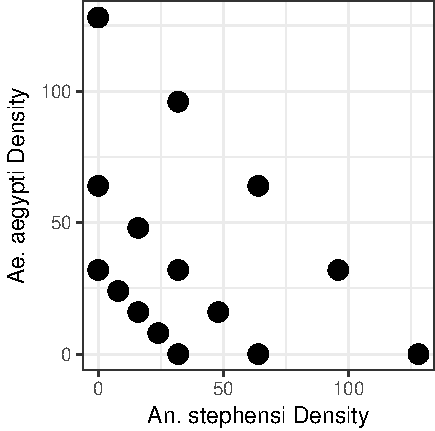
\includegraphics{manuscript_files/figure-latex/fig1-1.pdf}
\caption{Plot of density treatments used in experiment. Each group of
fifteen density treatments was repeated across five temperatures (16C,
20C, 24C, 28C, 32C).}
\end{figure}

Larvae were reared in 32 oz. glass jars with 250mL deionized water and
0.10g of pellet fish food (Hikari Cichlid Gold, baby size). Jars were
covered with a fine mesh and placed in Percival incubators with a daily
periodic fluctuation of 9C following the Parton-Logan equation,
characterized by a sine wave during the daytime and an exponential curve
during the nighttime \citep{parton1981}. Incubators were set to 80\%
relative humidity and 12:12 hour light:dark cycle.

To record information on mosquito survival and development rates, the
daily numbers, species, and sex of mosquitoes were recorded per species
ratio and temperature treatment.

To record measures of adult female fecundity and longevity, we offered a
subset of emerging mosquitoes a blood meal and followed individuals for
the span of their life. The subset encompassed mosquitoes emerging
during the period of peak emergence to ensure an adequate sample size
and a similarly aged cohort at the time of the blood feed (4-6 days
old). Adults were stored in reach-in Percival incubators at a constant
27C, 80\% relative humidity, 12:12 hr light:dark cycle and offered a
10\% sucrose solution \emph{ad libitum}. 48 hours prior to the blood
meal, the sucrose solution was replaced with deionized water, which was
removed 24 hours prior to the blood meal to encourage higher feeding
rates. Blood meals consisting of whole human blood were administered
through a water-jacketed membrance feeder kept at 38C.

Mosquitoes were allowed to feed for 20 minutes, after which blood fed
females were sorted into individual 50 mL plastic centrifuge tubes.
Moistened cotton was placed at the bottom of each tube, and covered with
a filter paper to collect eggs. Each tube was covered with a fine mesh
and kept in a walk-in incubator at the same environmental conditions
noted above. Individual females were monitored daily for mortality and
egg-laying events, after which the eggs were counted and the moistened
cotton and filter paper removed. Females continued to be kept as above
and offered a 10\% sucrose solution until death.

\subsection{Calculating Population Growth
Rates}\label{calculating-population-growth-rates}

We calculated the per capita population growth rate (Equation
\ref{eq:1}) per species ratio and temperature following
\citep{livdahl1984}:

\begin{equation} \label{eq:1}
r' = \frac{ln(\frac{1}{N_0}\sum_{x}^{ }{A_x}f(\bar{w_x}))}{D+\frac{\sum_{x}^{ }xA_xf(\bar{w_x})}{\sum_{x}^{ }A_xf(\bar{w_x})}}
\end{equation}

Where \(N_0\) is the initial number of female mosquitoes (assumed to be
50\% of the starting density), \(A_x\) is the number of mosquitoes
emerging on day \(x\), \(D\) is the time to reproduction following
emergence (assumed to be 14 days \citep{livdahl1991}), and
\(f(\bar{w_x})\) is the mean fecundity as measured by egg counts.
Because fecundity was only observed a subset of females from each
treatment, mean predicted fecundity from statistical models (described
below) was used for \(f(\bar{w_x})\). We exponentially transformed
\(r'\) to calculate population growth rates as \(\lambda\) in order to
solve for netatively infinite values.

\subsection{Statistical Analysis}\label{statistical-analysis}

Generalized linear mixed models (GZLMs) were used to investigate the
effects of interspecific densities, intraspecific densities, and
temperature on the proportion of females surviving to adulthood, adult
female fecundity, and population level growth rates. All models included
replicate as a random effect (intercept). Rescaled covariates were used
in models to account for differences in scale. For response variables
from the \emph{Ae. aegypti}, we fit a binomial GZLM (logit-link), a
zero-inflated negative binomial mixed-model, and a linear mixed model to
the survival, fecundity, and growth rates, respectively. \emph{An.
stephensi} had overall lower survival rates, leading to sparse,
zero-inflated data for fecundity and growth rates. Therefore, we fit a
GZLM with a binomial and logit link function, a negative binomial hurdle
model, and a linera mixed-effects hurdle model to the survival,
fecundity, and growth rates, respectively. The majority of mosquito
life-history traits have a non-linear relatioship with temperature
\citep{mordecai2017}, and so second-order transformations were used when
visual inspection revealed quadratic relationships. Model selection was
conducted via manual forward step-wise AIC, and final models included
only signficant variables, as evaluated by 95\% confidence intervals.
Model residuals were inspected visually to test for violations of
assumptions of normality. Due to difficulty in visualizing raw
multi-dimensional data, model predictions were used to generate figures.

\section{Results}\label{results}

\subsection{Results}\label{results-1}

\begin{table}[]
\centering
\caption{Table of results from mixed models of \textit{Ae. aegypti} survival, fecundity, and per capita growth as a function of temperature, interspecific density and intraspecific densities. }
\label{ref:tab}
\begin{tabular}{lllll}
\textbf{}       & {\ul \textbf{Term}}           & {\ul \textbf{Estimate}} & {\ul \textbf{s.e.}} & {\ul \textbf{p-value}} \\
\hline
\textbf{Aedes Survival}  &                               &                         &                     &                        \\
                & (Intercept)                   & 2.7801691               & 0.15444343          & \textless0.001         \\
                & AeDensScale                   & -1.99257404             & 0.08363467          & \textless0.001         \\
                & Temperature                   & 0.09638817              & 0.70679854          & 0.892                  \\
                & Temperature\textasciicircum 2 & -3.83762892             & 0.51334119          & \textless0.001         \\
                & StDensScale                   & -0.60399277             & 0.29535243          & 0.041                  \\
                & StDensScale:TempNum           & 0.03404162              & 0.0124021           & 0.006                  \\
\hline
\textbf{Aedes Fecundity} &                               &                         &                     &                        \\
                & (Intercept)                   & 4.274                   & 0.072               & \textless0.001         \\
                & Aedes Density                 & -0.008                  & 0.001               & \textless0.001         \\
                & Temperature                   & -3.041                  & 0.654               & \textless0.001         \\
                & Temperature\textasciicircum 2 & -1.812                  & 0.657               & 0.006                  \\
\hline
\textbf{Aedes Growth}    &                               &                         &                     &                        \\
                & (Intercept)                   & 1.188817675             & 0.003108282         & \textless0.001         \\
                & AeDensScale                   & -0.057255404            & 0.00263072          & \textless0.001         \\
                & poly(TempScale, 2)1           & 0.300784779             & 0.016861466         & \textless0.001         \\
                & poly(TempScale, 2)2           & -0.158920057            & 0.016867225         & \textless0.001
\end{tabular}
\end{table}

\begin{table}[]
\centering
\caption{Table of results from mixed models of \textit{Ae. aegypti} survival, fecundity, and per capita growth as a function of temperature, interspecific density and intraspecific densities. }
\label{ref:tab2}
\begin{tabular}{lllll}
                             & {\ul \textbf{Term}}             & {\ul \textbf{Estimate}} & {\ul \textbf{s.e.}} & {\ul \textbf{p-value}} \\
\hline
\textbf{Stephensi Survival}  &                                 &                         &                     &                        \\
                             & (Intercept)                     & 1.938                   & 0.603               & 0.001                  \\
                             & StDensScale                     & -5.161                  & 0.818               & \textless0.001         \\
                             & AeDensScale                     & -6.287                  & 0.821               & \textless0.001         \\
                             & poly(TempScale, 2)1             & 24.258                  & 5.651               & \textless0.001         \\
                             & poly(TempScale, 2)2             & 6.452                   & 4.372               & 0.14                   \\
                             & StDensScale:poly(TempScale, 2)1 & -36.003                 & 9.160               & \textless0.001         \\
                             & StDensScale:poly(TempScale, 2)2 & -19.723                 & 6.738               & 0.003                  \\
                             & AeDensScale:poly(TempScale, 2)1 & -35.208                 & 9.594               & \textless0.001         \\
                             & AeDensScale:poly(TempScale, 2)2 & -16.790                 & 7.738               & 0.03                   \\
\hline
\textbf{Stephensi Fecundity} &                                 &                         &                     &                        \\
                             & Zero hurdle intercept           & -1.084                  & 0.241               & \textless0.001         \\
                             & NegBin Intercept                & 4.205                   & 0.096               & \textless0.001         \\
                             & Log(theta)                      & 1.621                   & 0.317               & \textless0.001         \\
\hline
\textbf{Stephensi Growth}    &                                 &                         &                     &                        \\
Zero hurdle                  & Intercept                       & 3.216                   & 0.807               & \textless0.001         \\
                             & AeDensScale                     & -5.471                  & 1.29                & \textless0.001         \\
                             & StDensScale                     & -2.896                  & 0.773               & \textless0.001         \\
LMM                          & Intercept                       & 1.019                   & 0.03                & \textless0.001         \\
                             & Temperature                     & 0.075                   & 0.027               & 0.009
\end{tabular}
\end{table}


\textbf{Survival}: Both species experienced differential survival across
experimental treatments, with \emph{Ae. aegypti} survival rates higher
than \emph{An. stephensi} survival rates in all regimes. However, only
\emph{Ae. aegypti} was significantly impacted by temperature (Table 1),
exhibiting a unimodal relationship with temperature, with the highest
survival peaking around 24C (Figure 2A). \emph{An. stephensi} survival
did not differ across temperature, but did significantly decrease with
increasing intraspecific and interspecific densities (Figure 2B), with
interspecific densities having a larger negative effect than
intraspecific densities (Table 2). The effect of \emph{An. stephensi}
density on \emph{Ae. aegypti} survival was temperature dependent, with a
stronger negative effect at cooler temperatures, gradually becoming a
positive effect at warmer temperatures (Fig. 2A).

\begin{figure}[htbp]
\centering
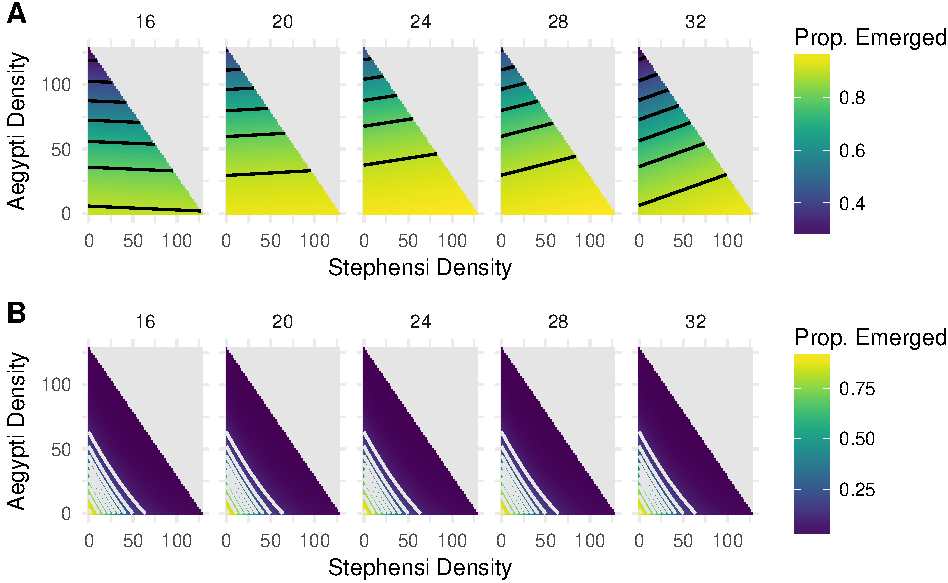
\includegraphics{manuscript_files/figure-latex/fig2-1.pdf}
\caption{Results from binomial GZLMs of species' densities (along the
axes) and temperature (by facet) on \emph{Ae. aegypti} (A) and \emph{A.
stephensi} (B) probability of survival to emergence. Contour lines
represent bins of 0.1.}
\end{figure}

\textbf{Fecundity}: Only \emph{Ae. aegypti} fecundity was significantly
affected by any density or temperature treatment. Due to low \emph{An.
stephensi} survival rates, the sample sizes of females with which to
measure fecundity was very small (with a median n=3), reducing the
statistical power to identify an effect. \emph{Ae. aegypti} fecundity
decreased with increasing intraspecific densities and increasing
temperatures (Fig. 3). Again, the relationship with temperature was
unimodal, with highest fecundity around 20C for all intraspecific
densities.

\begin{figure}[htbp]
\centering
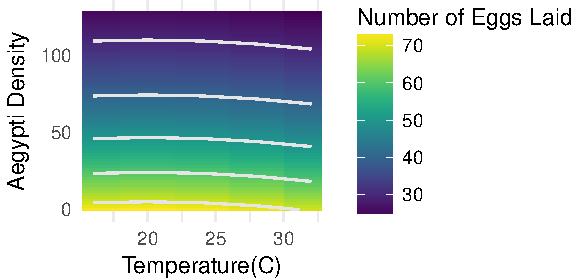
\includegraphics{manuscript_files/figure-latex/fig3-1.pdf}
\caption{\emph{Ae. aegypti} fecundity across temperature and
intraspecific density. Interspecific density had no significant effect
on fecundity. Contour lines represent bins of 10 eggs.}
\end{figure}

\textbf{Growth Rates}: When mosquito emergence and fecundity were
integrated into the per capita growth equation, \emph{Ae. aegypti}
population growth was positive for all levels of treatment and
densitites (Fig. 4A). \emph{An. stephensi}, had few instances of
positive growth (Fig. 4B), with many treatments resulting in no survival
to adulthood, and therefore no offspring at timestep \(t+1\). \emph{Ae.
aeygpti} growth rates decreased with increasing intraspecific densities
and had a unimodal relationship with temperature, peaking in the 28C
treatment. \emph{An. stephensi} growth rate was a function of all three
treatments, with inter- and intra-specific densities determining the
first stage of the hurdle model (e.g.~if growth was non-zero), and
temperature influencing growth rates of non-zero treatments (Table 2).
Growth rates decresed as either density increased, however the effect of
\emph{Ae. aegypti} densities was about two times as strong as that of
\emph{An. stephensi} densities (Table 2, Fig 4 B).

\begin{figure}[htbp]
\centering
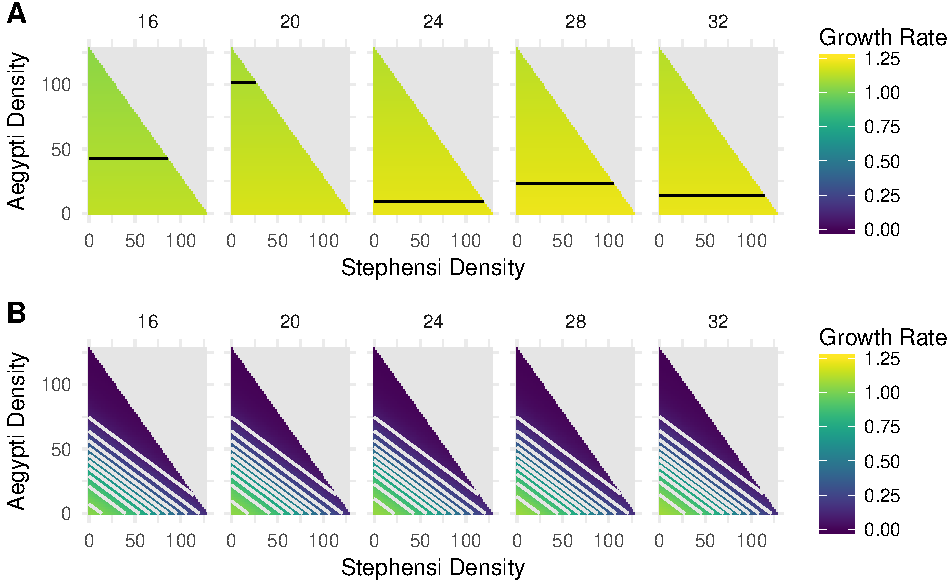
\includegraphics{manuscript_files/figure-latex/fig4-1.pdf}
\caption{\emph{Ae. aegypti} (A) and \emph{An. stephensi} (B) growth
rates across species densities (axes) and temperature (facet). Countour
lines represent bins of 0.1.}
\end{figure}



\section{Discussion}\label{discussion}

The context-dependence of biotic interactions is commonly seen in nature
\citep{chamberlain2014}, yet most studies of vector competition do not
incorporate this environmental variation in their evaluation of
competitive outcomes. Mosquitoes are particularly sensitive to
temperature variation, with implications for context-dependent
competition, population dynamics, and disease dynamics. We found that
the population growth rates of two mosquito species, \emph{Ae. aegypti}
and \emph{An. stephensi}, shifted with temperature and species
densities, however, temperature did not change the direction of the
species interaction on population growth rates.

In general, we found that \emph{Ae. aegypti} was more sensitive to
changes in temperature than \emph{An. stephensi}, with temperature
significantly influencing survival, fecundity, and per capita growth
rates. This is in agreement with many single-species studies, that have
found life history traits of \emph{Ae. aegypti} to be
temperature-dependent \citep{couret2014, yang2009, marinho2016}.
Interstingly, we found the effect of temperature on adult fecundity to
be unimodal, while other studies have female fecundity to have a
negative linear relationship with temperature \citep{lounibos2002a}.
This is likely due to our use of fluctuating temperatures, which result
in temperatures below and above the thermal minimum and maximum of
\emph{Ae. aegypti} thermal performance curves \citep{mordecai2017}. When
studied under fluctuating temperature regimes,
\citeyearpar{carrington2013} also found a non-linear relationship
between fecundity and temperature.

Our results suggest that \emph{Ae. aegypti} will outcompete \emph{An.
stephensi} across all environmental temperatures. However, we did find
that \emph{An. stephensi} had a negative effect on \emph{Ae. aegypti}
survival at lower temperatures, gradually becoming positive at higher
temperatures (Fig. 2A). The shift in direction from competition (-/-) to
predation (+/-) could be caused by the the increase in \emph{Ae.
aegypti} development rates with increasing temperature. At higher
temperatures, \emph{Ae. aegypti} develop into adults more quickly
\citep{farjana2011}, and are able to outcompete the still slowly
developing \emph{An. stephensi} for limited resources. In field-based
studies in Sub-saharan Africa, the presence of a competing
\emph{Anopheles} species have been shown to increase the development of
the cohabiting species, when the focal species already has a relatively
faster larval development rate \citep{paaijmans2009}. This may be due to
plasticity in development rate, with larvae developing more quickly in
the presence of a competitor.

Although \emph{An. stephensi} was less sensitive to environmental
temperature, its survival and growth rates were significantly impacted
by increases in both inter- and intra-specific densities. The effect of
interspecific competition was stronger than intraspecific competition on
both rates (Table 2). Following classical competition theory, species
co-existence arises when species limit themselves more than their
competitor (intraspecific \textgreater{}interspecific)
\citep{levins1968}. Therefore, across the temperature regimes in our
study, co-existence of both species in one container is unlikely.

However, both species exist in nature simultaneously
\citep{thomas2016, vikram2015}, suggesting that co-existence is
possible. This is further evidenced by the temporal overlap of dengue
and malaria cases in urban areas of India
\citep{telle2016, santos-vega2016a}. One explanation for this regional
coexistence in spite of local competitive exclusion may be due to
habitat partitioning across temperature regimes. Our study found that
\emph{An. stephensi} was most competitive at cooler temperatures and low
interspecific densities (Fig. 4A). In the field, \emph{An. stephensi}
are most often found in large cement water tanks \citep{thomas2016},
which exhibit a cooler thermal environment than the preferred
small-container habitat of \emph{Ae. aegypti} \citep{cator2013}, and,
due to their large size, have relatively lower densities of mosquito
larvae. This fine-scale habitat partitioning has been observed in the
\emph{Ae. aegypti}-\emph{Ae. albopictus} system, in which \emph{Ae.
aegypti} is the weaker competitor, however there are no
context-dependent differences in competitive strength
\citep{juliano2004}. However, there is variation in competition amongst
geographically-distinct strains of both species \citep{leisnham2010},
and in the species' ability to survive dessication at the egg stage
\citep{juliano2002}. This suggests that regional co-existence may be a
result of genetic variation or species' advantages at non-competitive
life-stages.

We found that \emph{An. stephensi} is outcompeted by \emph{Ae. aegypti}
across a range of temperature treatments. Co-existence of both species
at a local scale is therefore unlikely. However, the magnitude of the
effect of competition is dependent on temperature, and therefore, across
a thermally heterogeneous landscape, co-existence may be possible at
larger scales. We found all species' demographic rates to change as a
function of species density, identifying density-dependence as an
important control on population dynamics. Models of mosquito-borne
disease rarely include effects of species density at the larval stage,
particularly competition, \citep{reiner2013}, and therefore may be
incorrectly estimating population growth rates of these two species.
Further, our experiment was conducted with only one strain of each
species, and followed cohorts for one generation time, without
calculating hatch rate success. Future work should explore the
possibility of genotype x genotype x environment interations and expand
the study over multiple generations.




\newpage
\singlespacing
\renewcommand\refname{References}
\bibliography{references}

\end{document}
